\section{Uživatelská příručka}

\subsection{Požadavky}
Pro spuštění aplikace je potřeba mít nainstalovaný python 3.

\subsection{Spuštění ze zdrojových kódů}

Projekt využívá pro správu zavíslostí nástroj Poetry, který je možné nainstalovat
pomocí příkazu:
\begin{lstlisting}
pip install poetry
\end{lstlisting}

Následně pomocí poetry nainstalujeme všechny závislosti definované v souboru \emph{pyproject.toml}
pomocí příkazu:
\begin{lstlisting}
poetry install
\end{lstlisting}

Vlatní aplikaci můžeme spustit pomocí příkazu (parametry viz níže):
\begin{lstlisting}
poetry run start
\end{lstlisting}

\subsection{Spuštění z wheel balíčku}
K dispozici je také \emph{.wheel} soubor \emph{hmm\_stock\_forecast-1.0-py3-none-any.whl},
který můžeme nainstalovat id bez Poetry pomocí příkazu:
\begin{lstlisting}
python -m pip install hmm_stock_forecast-1.0-py3-none-any.whl
\end{lstlisting}
A následně spustit (parametry viz níže):
\begin{lstlisting}
python -m hmm_stock_forecast.main
\end{lstlisting}

\subsection{Parametry programu}
Aplikace očekává následující parametry:
\begin{itemize}
    \item -t ticker akciového titulu (např. AAPL)
    \item -f cesta k csv souboru (4 sloupce: Open, Low, High, Close)
    \item -s datum počátku dat, která se mají stáhnout
    \item -e datum konce dat, která se mají stáhnout
    \item -w velikost okna viz výše (defaultně 120)
    \item -m typ modelu:
    \begin{itemize}
        \item HMM - naše implementace modelu (defaultně)
        \item pomegranate - využití modelu knihovny pomegranate
    \end{itemize}
\end{itemize}
Spuštění je tedy možné buď s -f nebo -t, v tom případě jsou povinné i datumy pro stažení dat z yahoo finance.
Na obrázku \ref{fig:output} je vidět výstup aplikace.

\begin{figure}[h]
    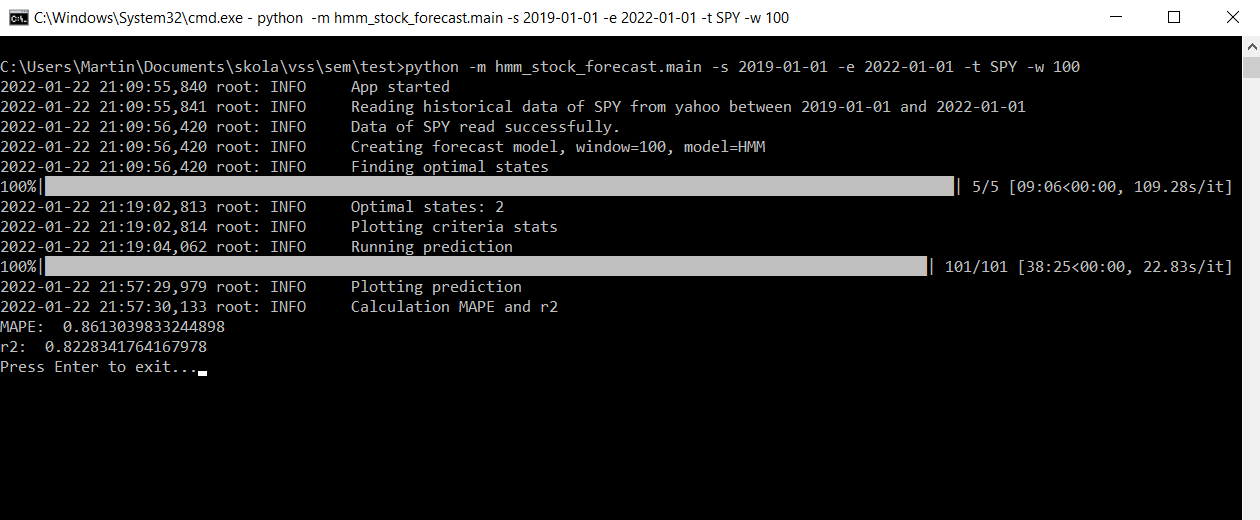
\includegraphics[width=1\textwidth]{img/output}
    \caption{Výstup aplikace}
    \label{fig:output}
\end{figure}

\clearpage
